\section{Phase-field approach to brittle fracture}
\label{sec:pf}

This section introduces the phase-field approach to fracture as a
regularisation of the revisited Griffith theory by Francfort and Marigo.
Extensions to more general class of damage gradient models as well as
extensions to take into account unilateral effects are then discussed.

The various numerical strategies to implement the irreversibility constraint are described.

Then, we introduce some common numerical scheme to solve both the
mechanical equilibrium and the phase-field problem.

We conclude by some showcases of our current implementation of the
phase-field method in \texttt{Cast3M} and some early work on the acceleration
of the staggered schemes with \texttt{FEniCS}.

\subsection{Some words on Griffith's theory of brittle fracture}

In this paragraph, one considers a solid \(\Omega\) containing a crack
\(\Gamma\). The material is assumed to be linear elastic.

In the absence of applied forces, the Griffith theory of brittle
fracture states that \cite{francfort_revisiting_1998}:

\begin{itemize}
    \item The following inequality holds:
    \[
    G \leq G_{c}
    \]
    where \(G=-\derivtot{}{\Gamma}\paren{\displaystyle\int_{\Omega\backslash\Gamma}\,\Frac{1}{2}\,\tepsilonto\,
    \colon\,\fotensor{D}\,\colon\,\tepsilonto}\,\dtot\,V\)
    is the elastic energy release rate of the whole structure
    (\(\fotensor{D}\) is the stiffness matrix) and
    \(G_{c}\) is fracture energy \(G_{c}\).
    \item That a crack propagation may not occur if the energy release rate is
    strictly lower than the fracture energy.
\end{itemize}

% - The following inequality holds:
%   \[
%   G \leq G_{c}
%   \]
%   where:
%   -
%     \(G=-\derivtot{}{\Gamma}\paren{\displaystyle\int_{\Omega\backslash\Gamma}\,\Frac{1}{2}\,\tepsilonto\,\colon\,\fotensor{D}\,\colon\,\tepsilonto}\,\dtot\,V\)
%     is the elastic energy release rate of the whole structure
%     (\(\fotensor{D}\) is the stiffness matrix) and
%   - \(G_{c}\) is fracture energy \(G_{c}\).
% - That a crack propagation may not occur if the energy release rate is
%   strictly lower than the fracture energy.

When taking the irreversibility of the crack propagation, the Griffith
theory can be summarised by the following Kuhn-Tucker relations:

\[
\left\{
\begin{aligned}
\dot{\Gamma}&\geq 0\\
G &\leq G_{c}\\
\paren{-G +G_{c}}\dot{\Gamma}&=0
\end{aligned}
\right.
\]

The Griffith theory has three main flaws \cite{francfort_vers_2002}:

\begin{itemize}
    \item Crack initiation can't be described, as the energy release rate tends
    to zero with the crack surface. Thanks to classical Irwin relations,
    one sees that the energy release rate is related to the stress field
    singularities.
    \item Determination of the crack path requires additional criteria.
    \item Crack propagation must be stable.
\end{itemize}

\subsection{Brittle fracture as an energy minimisation problem}

The variational approach to fracture takes its grounds in the work of
Francfort and Marigo which recasted the Griffith theory into an enery
minimization problem \cite{francfort_revisiting_1998, francfort_vers_2002}:

\begin{equation}
    \label{eq:phase_field:marigo}
    \paren{\ets{\vec{u}},\ets{\Gamma}}=
    \underset{
    \begin{aligned}
    \vec{u}^{\star}&\in\text{C.A.}\\
    \bts{\Gamma}&\subset\Gamma^{\star}
    \end{aligned}
    }{\argmin{}}
    \int_{\Omega\backslash\Gamma^{\star}}\,\Frac{1}{2}\,\tepsilonto\paren{\vec{u}^{\star}}\,\colon\,\fotensor{D}\,\colon\,\tepsilonto\paren{\vec{u}^{\star}}\,\dtot\,V + G_{c}\,\Gamma^{\star}
\end{equation}

Problem \eqref{eq:phase_field:marigo} is however not tractable with standard
numerical methods
\cite{bourdin_numerical_2000, chambolle_approximation_2018}, in particular
the commonly used finite element method. For this reason, regularised
versions were developed.

\subsubsection{Regularisation of Problem \eqref{eq:phase_field:marigo} as a non local damage behaviour}

Following mathematical works of
\cite{ambrosio_approximation_1990}, the regularization proposed by Bourdin \textit{et
al.} relies on the following lagrangian \cite{bourdin_numerical_2000}:

\begin{equation}
    \label{eq:phase_field:Bourdin_Lagrangian}
    \mathcal{L}(\vec{u},d) =
   \int_{\Omega} \rho\psi\paren{\tepsilonto,d} \dtot V
   + \dfrac{G_c}{c_w} \int_{\Omega}\paren{\Frac{w(d)}{l} + l \|\vec{\nabla} d\|^2}\dtot V
   - \mathcal{W}_{\mathrm{ext}}(\vec{u})
\end{equation}

in which:

\begin{itemize}
    \item \(d\in[0;1]\) is the damage variable, *i.e.* a continuous field
    representing the crack in a *smeared* fashion. The crack position is
    lies in the isovalue (\(d=1\)).
    \item \(\rho\psi\) is the part of the free energy coupling elasticity and
    damage. \(\rho\psi\) is the product a degradation function
    \(g\paren{d}\) and the free energy \(\rho\psi^{\mathrm{el}}\) of an
    elastic undamaged material:
    \[
    \begin{aligned}
    \rho\psi\paren{\mathrm{el},d}&=g\paren{d}\,\rho\psi^{\mathrm{el}}\paren{\mathrm{el}}\\
    \rho\psi^{\mathrm{el}}\paren{\mathrm{el}}&=\dfrac{1}{2}\,\mathrm{el}\,\colon\,\fotensor{D}\,\colon\,\mathrm{el}
    \end{aligned}
    \]
    \item \(g(d)\) is assumed to be a strictly-decreasing function which satisfies
    \(g\paren{0}=1\) and \(g\paren{1}=0\).
    \item \(l\) is a small regularization length-scale parameter.
    \item \(w(d)\) a strictly-increasing function.
    \item \(c_w\) a numerical constant associated with \(w\).
\end{itemize}

% - \(d\in[0;1]\) is the damage variable, *i.e.* a continuous field
%   representing the crack in a *smeared* fashion. The crack position is
%   lies in the isovalue (\(d=1\)).
% - \(\rho\psi\) is the part of the free energy coupling elasticity and
%   damage. \(\rho\psi\) is the product a degradation function
%   \(g\paren{d}\) and the free energy \(\rho\psi^{\mathrm{el}}\) of an
%   elastic undamaged material:
%   \[
%   \begin{aligned}
%   \rho\psi\paren{\mathrm{el},d}&=g\paren{d}\,\rho\psi^{\mathrm{el}}\paren{\mathrm{el}}\\
%   \rho\psi^{\mathrm{el}}\paren{\mathrm{el}}&=\dfrac{1}{2}\,\mathrm{el}\,\colon\,\fotensor{D}\,\colon\,\mathrm{el}
%   \end{aligned}
%   \]
%   <!-- \[
%   \begin{aligned}
%   \rho\psi\paren{\tepsilonto,d}&=g\paren{d}\,\rho\psi^{\mathrm{el}}\paren{\tepsilonto}\\
%   \rho\psi^{\mathrm{el}}\paren{\tepsilonto}&=\dfrac{1}{2}\,\tepsilonto\,\colon\,\fotensor{D}\,\colon\,\tepsilonto
%   \end{aligned}
%   \] -->
%   \(g(d)\) is assumed to be a strictly-decreasing function which satisfies
%   \(g\paren{0}=1\) and \(g\paren{1}=0\).
% - \(l\) is a small regularization length-scale parameter.
% - \(w(d)\) a strictly-increasing function.
% - \(c_w\) a numerical constant associated with \(w\).

In such an approximation, the crack surface is smeared in a location
band whose width is of the order of the characteristic length \(l\).

As regards the fracture energy density, two choices originating from the
work of Ambrosio and Tortorelli (AT) are widely used, namely:

\begin{itemize}
    \item AT2 model: \(w(d) = d^2, c_w=2\).
    \item AT1 model: \(w(d) = d, c_w=\dfrac{8}{3}\). The main advantage of the AT1 model is that it exhibits an elastic domain prior damage.
\end{itemize}

The constant $c_w$ is chosen so that analytical localized solution
profiles correspond to a dissipated energy precisely equal to $G_c$.

The evolution of the displacement \(\vec{u}\) and damage field \(d\)
satisfies the minimisation principle:

\begin{equation}
    \label{eq:phase_field_lagrangian}
    \paren{\ets{\vec{u}},\ets{d}}=
    \underset{
    \begin{aligned}
    \vec{u}^{\star}&\in\text{C.A.}\\
    d^{\star}&\geq\bts{d}
    \end{aligned}
    }{\argmin{}}\,\mathcal{L}(\vec{u}^{\star},d^{\star})
\end{equation}

Problem \eqref{eq:phase_field_lagrangian} typically defines a non local damage
model in the framework of generalised standard materials (see section
\ref{sec:phase_field:lorentz_variational_framework} below). This non local
model can be viewed as a regularisation of a local damage model.

The Lagrangian \eqref{eq:phase_field:Bourdin_Lagrangian} uses the first
gradient of damage, but higher order theories may be built as in of the
work of Verhoosel et al. \cite{verhoosel_isogeometric_2011}.

\subsubsection{About \(\Gamma\)-convergence}

Several works have shown that the solutions of
\eqref{eq:phase_field_lagrangian} converge in the sense of the so-called
\(\Gamma\)-convergence, to the solution of the initial Problem
\eqref{eq:phase_field:marigo} in some specific cases. For example,
\cite{bourdin_numerical_2000} studied the anti-plane shear case.

Those results bridges the conceptual gap between the global approach of
fracture based on Griffith' theory and the local approach to fracture, a
least for a certain class of non local models.

\paragraph{\(\Gamma\)-convergence and the search of minima}

The relationship between the smeared model and its parent discrete
model is corroborated by the proof of the \(\Gamma\)-convergence result,
even if it should be emphasized that \(\Gamma\)-convergence considers
global minima only, whereas fracture mechanics typically deals
with local minima \cite{freddi_regularized_2010}.

\subsubsection{Unilateral effects}
\label{sec:phase_field:unilateral_effects}

The Lagrangian \(\mathcal{L}(u,d)\) can be modified to express the
effect of crack closure, \textit{i.e.} the so-called unilateral effect.

The description of unilateral effects commonly starts by a decomposition
of the elastic energy of an undamaged material into a tensile part
\(\rho\psi^{\mathrm{el}}_{+}\) and a compressive part part
\(\rho\psi^{\mathrm{el}}_{-}\).

The degradation function is then only applied on the positive part, as
follows:

\[
\rho\psi^{\mathrm{el}}\paren{\tepsilonto,d}=g\paren{d}\,\rho\psi^{\mathrm{el}}_{+}\paren{\tepsilonto}+\rho\psi^{\mathrm{el}}_{-}\paren{\tepsilonto}
\]

Here are two classical choices of this decomposition:

\begin{itemize}
    \item A volumetric/deviatoric splitting, as introduced by Amor et al.
    \cite{amor_regularized_2009}:
    \[
    \left\{
    \begin{aligned}
      \rho\psi^{\mathrm{el}}_{+}\paren{\tepsilonto} &= \dfrac{1}{2}\kappa \ppart{\Tr{\tepsilonto}}^2 + \mu
      \dev\paren{\tepsilonto}\,\colon\,\dev\paren{\tepsilonto}\\
      \rho\psi^{\mathrm{el}}_{-}\paren{\tepsilonto} &=
      \dfrac{1}{2}\kappa \npart{\Tr{\tepsilonto}}^2
    \end{aligned}
    \right.
    \]
    where $\kappa=\lambda+\dfrac{2}{3}\mu$ stands for the compression modulus.
    \item Spectral decomposition, as used by Miehe in the context of the
    variational fracture \cite{miehe_phase_2010}:
    \begin{equation}
        \label{eq:phase_field:spectral_decomposition}
        \left\{
        \begin{aligned}
        \rho\psi^{\mathrm{el}}_{+}\paren{\tepsilonto} &= \dfrac{\lambda}{2}\, 
        \ppart{\Tr{\tepsilonto}}^2 + \mu
        \ppart{\tepsilonto}\,\colon\,\ppart{\tepsilonto}\\
        \rho\psi^{\mathrm{el}}_{-}\paren{\tepsilonto} &= \dfrac{\lambda}{2}\, 
        \npart{\Tr{\tepsilonto}}^2 + \mu
        \npart{\tepsilonto}\,\colon\,\npart{\tepsilonto}\\
        \end{aligned}
        \right.
    \end{equation}
\end{itemize}

See also \cite{chambolle_approximation_2018} for some \(\Gamma\)-convergence
results of these models to an extension of Problem \eqref{eq:phase_field:marigo}
taking non interpenetration of the crack surfaces.

\subsubsection{Crack nucleation}
\label{sec:phase_field:crack_nucleation}

Many authors tried to identify the characteristic length \(l\) as a
material parameter and link it to some observable quantities, such as
the tensile strength \(\sigma_{y}\) is the tensile strength.

\[
\begin{aligned}
\sigma_{y}&=\sqrt{\dfrac{3\,E\,G_{c}}{8\,l}}&\text{(AT1)}\\
\sigma_{y}&=\dfrac{9}{16}\sqrt{\dfrac{E\,G_{c}}{3\,l}}&\text{(AT2)}\\
\end{aligned}
\]

This approach has been criticized recently in \cite{kumar_revisiting_2020} :
since $l$ becomes a material parameter, the finite element study of some
materials becomes mesh-size dependent if $l$ is too large or too small
with respect to the element size. Moreover, tying $l$ to the single
parameter $\sigma_y$ ignores all other points of the strength surface,
and many loading paths different from pure traction are thus eluded.

\subsubsection{Lorentz' variational framework}
\label{sec:phase_field:lorentz_variational_framework}

Formulation \eqref{eq:phase_field_lagrangian} fits nicely into the variational
framework introduced by Lorentz et al., on the bases established by
Germain et al.
\cite{germain_continuum_1983, lorentz_variational_1999, lorentz_analysis_2003, forest_localization_2004}.
This framework allows properly building various extensions:

\begin{itemize}
    \item unilateral effects, as depicted in Section
    \ref{sec:phase_field:unilateral_effects}.
    \item cohesive fracture, see
    \cite{lorentz_convergence_2011, lorentz_nonlocal_2017}.
    \item finite strain modelling.
    \item coupling with other dissipative phenomena (viscoplasticity,
    plasticity, etc.). See for example
    \cite{zhang_modelisation_2016, crabbe_gradient_2018}.
\end{itemize}

In particular, the \texttt{ENDO\_SCALAIRE} damage behaviour corresponds
to the choice \cite{edf_loi_2011}:

\begin{itemize}
    \item \(g(d)=\paren{\dfrac{1-d}{1+\gamma\,d}}^{2}\) with
    \(\gamma=\dfrac{3\,E\,G_{c}}{2\,\sigma_{y}^{2}\,l}-1\) where
    \(\sigma_{y}\) is the tensile strength.
    \item \(w(d) = d\) and \(c_w=\dfrac{8}{3}\), *i.e.* the same choice as for
    the AT1 model.
\end{itemize}

\cite{lorentz_convergence_2011} shows how this behaviour converges to a
cohesive zone model when the characteristic length tends to \(0\) in
\(1D\), while results in \(2D\) may be found in
\cite{cuvilliez_transition_2011}.

\subsection{Numerical strategies}

The reader may refer of Gerasimov and De Lorenzis review which provides
a comprehensive overview of the various numerical approaches available
in the literature \cite{gerasimov_numerical_2020}.

\subsubsection{Weak forms}

Variation of Equation \eqref{eq:phase_field_lagrangian} with respect to the
displacement fields yields the classical principle of virtual work:

\begin{equation}
    \label{eq:phase_field:d}
    \int_\Omega \paren{\deriv{\rho\psi}{d} d^{\star}+\dfrac{G_c}{c_w}\paren{\dfrac{1}{l}\,\derivtot{w}{d}\,d^{\star} + 2\,l \vec{\nabla} d\, \cdot\, \vec{\nabla} d^{\star}}} \,\dtot\,V = 0
\end{equation}

If we neglect the irreversibility constraint, variation of Equation
\eqref{eq:phase_field_lagrangian} with respect to the damage field yields:

\begin{equation}
    \label{eq:phase_field:pvw}
        \begin{aligned}
            \int_{\Omega} \frac{\partial \rho \psi^{e}}{\partial \tepsilonto} : \tepsilonto (\vec{u}^{\star}) dV = \mathcal{W}_{ext}(\vec{u}^{\star})
        \end{aligned}
\end{equation}

\paragraph{Analogy with the transient heat equation}

When the degradation function is quadratic, Equation
\eqref{eq:phase_field:d} is formally equivalent to the
transient heat equation after being discretized
using a simple backward Euler algorithm.
This analogy is the basis of the implementations that we developed
in \texttt{Cast3M}
\cite{helfer_modelisation_2017, helfer_phase-field_2018, lu_schema_2019}.

\subsubsection{Treatment of the irreversibility constraint}

\paragraph{Constrained minimisation}

Many implementation based on the \texttt{FEniCS} solvers
\cite{alessi_gradient_2015, crabbe_etudes_2017, farrell_linear_2017, bleyer_phase-field_2020}
relies on the \texttt{PETScTAOSolver} optimisation algorithm which allows
finding the solution of the following convex problem:

\[
  \ets{d} = \underset{d^{\star}\geq\bts{d}}{\argmin{}}\, \mathcal{L}\paren{\vec{u},d^{\star}}
\]

where the displacement field \(\vec{u}\) is assumed to be known. This
kind of problem arises naturally when solving Problem
\eqref{eq:phase_field_lagrangian} using a staggered approach, as discussed in
Section \ref{sec:phase_field:staggered_resolution}.

This solver is interfaced by the \texttt{MFrontOptimisationProblem} of the
\texttt{mgis.fenics} python module
\cite{bleyer_overview_2020, bleyer_phase-field_2020} which is part of the
\texttt{MGIS} project \cite{helfer_mfrontgenericinterfacesupport_2020}.

\paragraph{Penalisation}

A comprehensive review of penalisation methods to enforce the
irreversibility condition is given in \cite{gerasimov_penalization_2019}.

\paragraph{Lagrange multipliers and active sets}

\cite{heister_primal-dual_2015, jodlbauer_parallel_2020}.

The use of Lagrange multipliers is the basis of the implementation that
we proposed in \cite{helfer_phase-field_2018}. An approximated treatment,
based on the postdoctoral work of Ye Lu, is discussed in Section
\ref{sec:phase_field:ye_lu_irreversibility}.

\paragraph{Miehe approach \cite{miehe_phase_2010}}

In this section, the specific choice of the free energy is considered:

\begin{equation}
    \rho\psi\paren{\tepsilonto,d}=\paren{1-d}^{2}\,\rho\psi^{\mathrm{el}}_{+}\paren{\tepsilonto}+\rho\psi^{\mathrm{el}}_{-}\paren{\tepsilonto}
\end{equation}
%
%
%
where \(\rho\psi^{\mathrm{el}}_{+}\) and
\(\rho\psi^{\mathrm{el}}_{-}\) are given by the Spectral Decomposition
\eqref{eq:phase_field:spectral_decomposition}.

Departing from the variational framework presented here, Miehe proposed
a different treatment of the irreversibility constraint, which consists
in the following modification of Equation \eqref{eq:phase_field:d}
\cite{miehe_phase_2010}:

\[
\int_\Omega \paren{-\paren{1-d}\mathcal{H}\widehat{d}+\dfrac{G_c}{c_w}\paren{\dfrac{1}{l}\,\derivtot{w}{d}\,d^{\star} + 2\,l \vec{\nabla} d\, \cdot\, \vec{\nabla} d^{\star}}} \,\dtot\,V = 0
\]

where \(\mathcal{H}\) is an history field holding the maximum value of
the (undamaged) elastic energy:

\[
\mathcal{H}=\underset{\tau<t}{\max}\, \rho\psi^{\mathrm{el}}_{+}\paren{\tepsilonto\paren{\tau}}
\]

Contrary to common beliefs in the litterature, this approach is not
equivalent to Problem \eqref{eq:phase_field_lagrangian}
\cite{gerasimov_numerical_2020}.

However, Miehe's proposal changes the nature of the problem to be solved
from a variational inequality to a variation equality which is:

\begin{itemize}
    \item much easier to implement or to introduce in standard finite
    element solver.
    \item much more efficient numerically.
\end{itemize}

This explains the success of this proposal which is the basis of most
works made in the phase-field approach of fracture. However, though Miehe's approach proves to be efficient for monotonic loadings, no results are provioded for non-monotonic loadings, and this approach needs be tested in such a situation.

\paragraph{Ye Lu' treatment of irreversibility \cite{lu_schema_2019}
\label{sec:phase_field:ye_lu_irreversibility}}

In an attempt to accelerate the treatment of the irreversibility
constraint using Lagrange multipliers, Ye Lu proposed an approximate
treatment of the irreversibility constraint:

\begin{equation}
    \label{eq:phase_field:ye_lu}
    \ets{d} = \underset{d^{\star}\geq\bts{d}}{\argmin{}}\, \mathcal{L}\paren{\vec{u},d^{\star}}
\end{equation}

where the displacement field \(\vec{u}\) is again assumed to be known.

Problem \eqref{eq:phase_field:ye_lu} is solved iteratively. At each iteration,
a Dirichlet condition, enforcing the constraint \(d^{(i)}=\bts{d}\), is
added to each node which does not respect the condition
\(d^{(i)}\geq\bts{d}\)w. Contrary to the active set algorithm, this
constraint is not removed during the iterations. Iterations are stopped
when every node satisfies the irreversibility constraint.

Ye Lu observed a significant decrease of the computational time when
compared to the use of the active set method, as implemented in
\texttt{Cast3M}.

Moreover, the approximated treatment of the irreversibility constraint
seems to be compensated by the fact that the Problem
\eqref{eq:phase_field:ye_lu} is part of a staggered approach which is described
in Section \ref{sec:phase_field:castem_implementation}. Although no proof can
be established that the converged solution of this staggered approach
with this approximated treatment of the irreversibility is equivalent of
a rigorous resolution of Problem \eqref{eq:phase_field_lagrangian}, numerical
results are encouraging \cite{lu_schema_2019}.

\subsubsection{Monolithic resolution}

\begin{figure}[H]
  \centering
  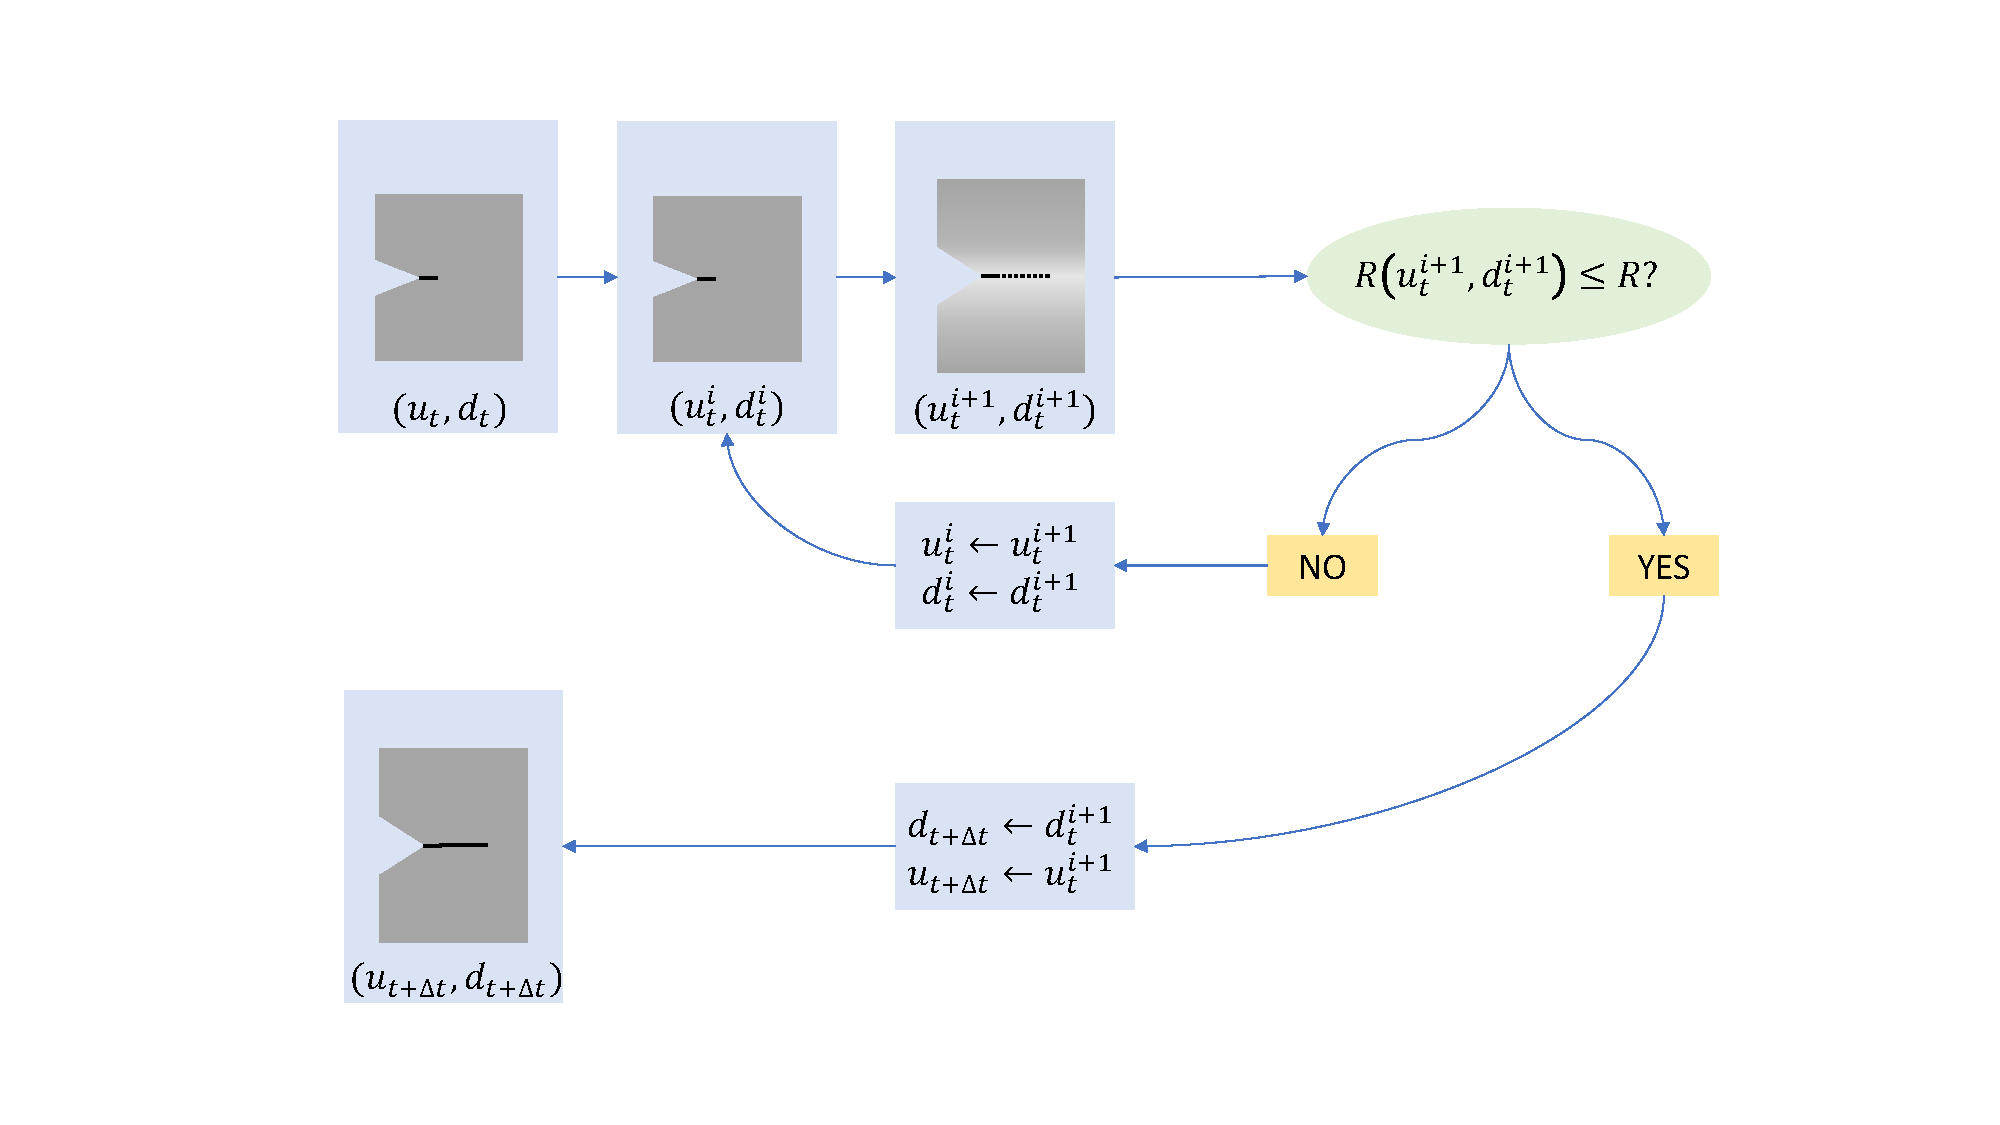
\includegraphics[width=10.cm]{../chapter_00_introduction/figures/monolithic-resolution.pdf}
  \caption{Illustration of the monolithic resolution of Problem \eqref{eq:phase_field_lagrangian}}
  \label{fig:hho:phase_field:monolithic_scheme}
\end{figure}

% ![Illustration of the monolithic resolution of Problem @eq:phase_field_lagrangian.](img/phase-field/monolithic-resolution.pdf){#fig:hho:phase_field:monolithic_scheme}

Monolithic resolutions solves both the phase-field and the mechanical
problem at the same time (see Figure
\ref{fig:hho:phase_field:monolithic_scheme}). When it converges, the
monolithic approach is very fast but, due to the non-convexity of the
Lagrangian \eqref{eq:phase_field:Bourdin_Lagrangian}, the standard Newton
generally fails to converge. Thus, globalisation or arc-length methods
are required \cite{wick_modified_2017, edf_modelisation_2019}. Good results
have been reported with quasi-Newton methods
\cite{wu_bfgs_2020, wu_comprehensive_2020}. In \cite{farrell_linear_2017}, a
staggered scheme is used to get close to the solution and a monolithic
approach is then used to make the final steps toward convergence.

\subsubsection{Staggered resolution}
\label{sec:phase_field:staggered_resolution}

Staggered resolutions are based on the idea of solving Problem
\eqref{eq:phase_field_lagrangian} alternatively:

\begin{itemize}
    \item for the displacement field (at constant damage field):
    \begin{equation}
        \label{eq:phase_field:problem_u}
        \vec{u} = \underset{\vec{u}^{\star}\in\text{C.A.}}{\argmin{}}\, \mathcal{L}\paren{\vec{u}^{\star},d_\mathrm{fixed}}
    \end{equation}
    \item for the damage field (at constant displacement field):
    \begin{equation}
        \label{eq:phase_field:problem_d}
        d = \underset{d^{\star}\geq\bts{d}}{\argmin{}}\, \mathcal{L}\paren{\vec{u}_\mathrm{fixed},d^{\star}}
    \end{equation}
\end{itemize}

Note that both Problems \eqref{eq:phase_field:problem_u} and
\eqref{eq:phase_field:problem_d} are convex.

\paragraph{Alternate minimisation}

\begin{figure}[H]
  \centering
  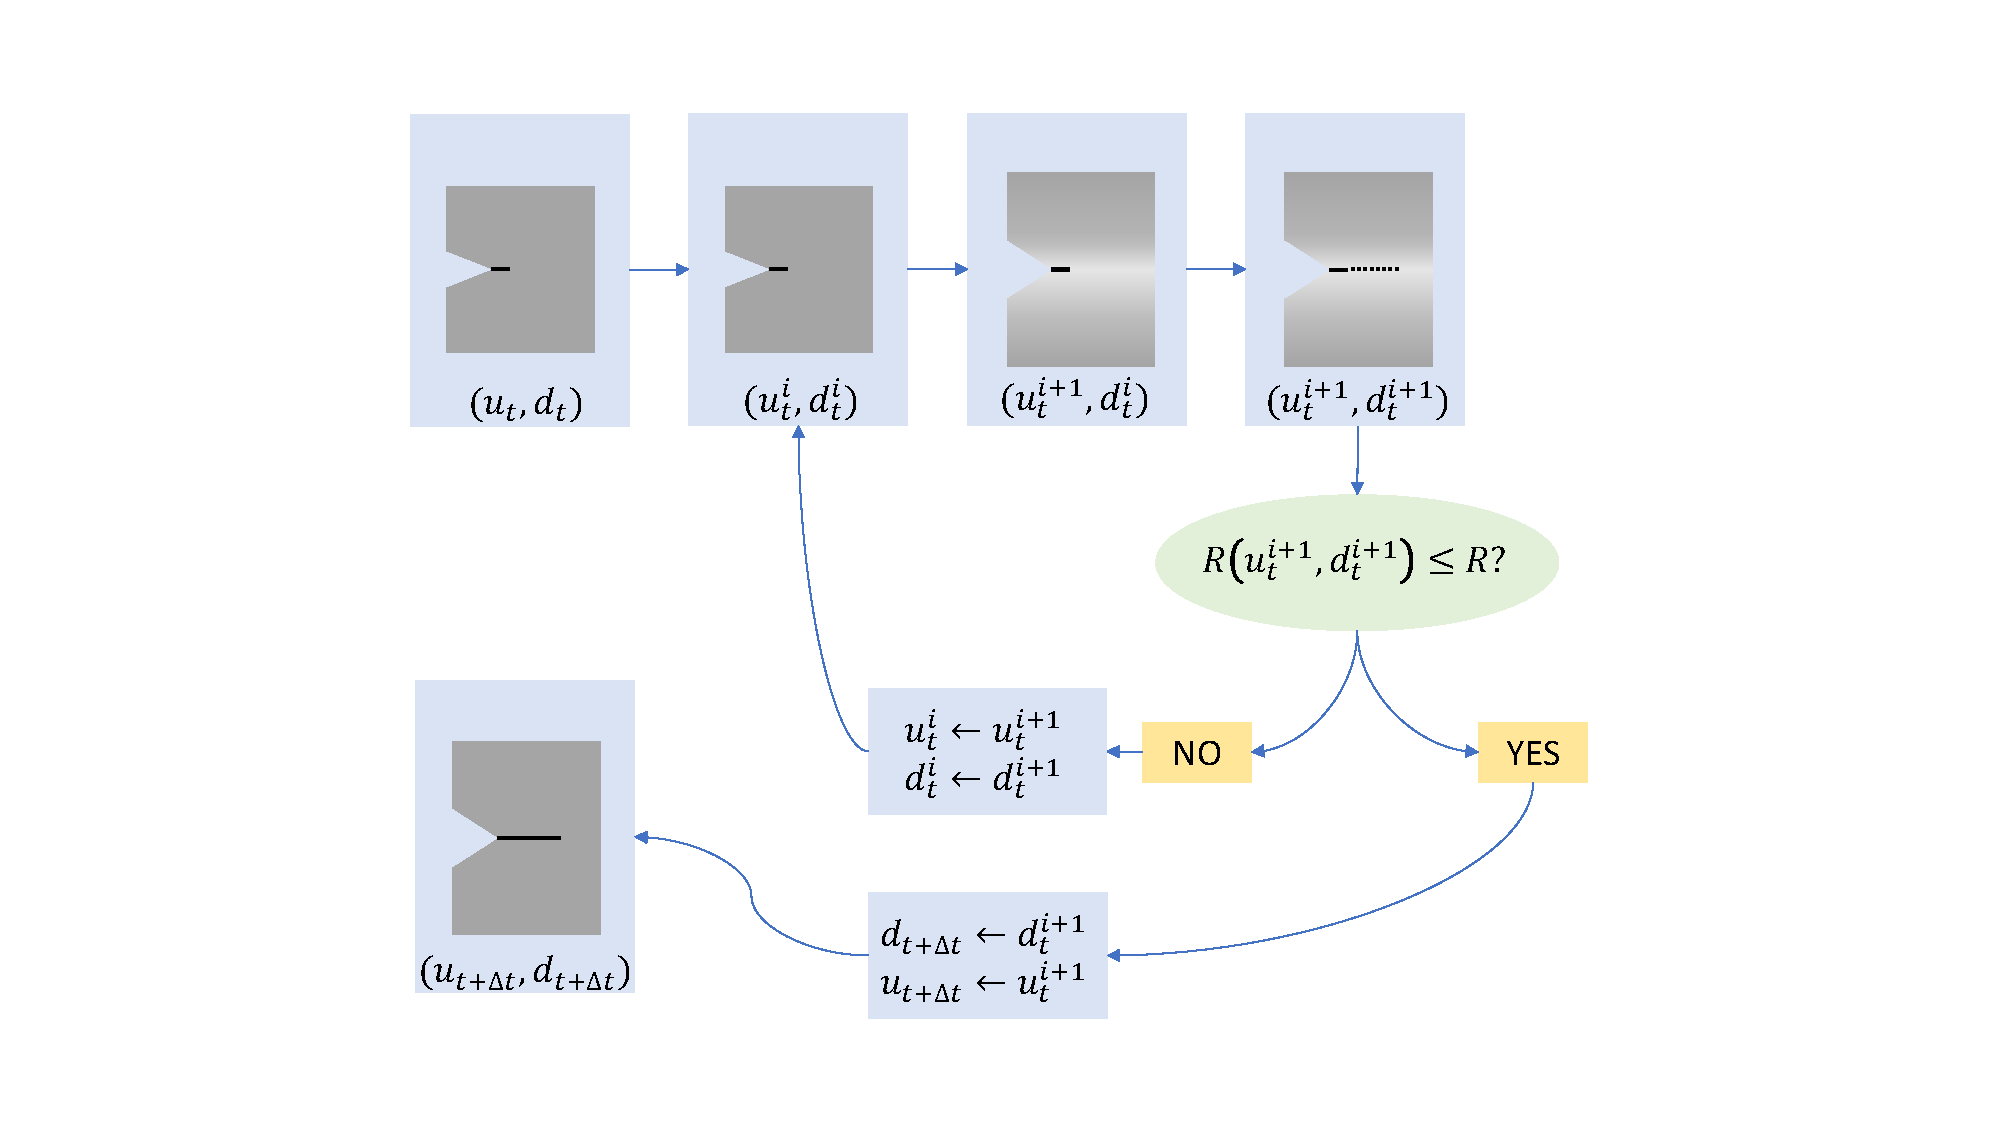
\includegraphics[width=10.cm]{../chapter_00_introduction/figures/alternate-minimisation-resolution.pdf}
  \caption{Illustration of the alternate minimisation algorithm applied to Problem \eqref{eq:phase_field_lagrangian}}
  \label{fig:hho:phase_field:alternate_minimisation}
\end{figure}

% ![Illustration of the alternate minimisation algorithm applied to Problem @eq:phase_field_lagrangian.](img/phase-field/alternate-minimisation-resolution.pdf){#fig:hho:phase_field:alternate_minimisation}

The alternate minimisation algorithm, introduced by \textit{Bourdin at al.}
\cite{bourdin_numerical_2000}, uses a fixed point algorithm to find a pair
\(\ets{\vec{u}},\ets{d}\) which satisfies both Problems
\eqref{eq:phase_field:problem_u} and \eqref{eq:phase_field:problem_d}, \textit{i.e.} is a
solution of the initial Problem \eqref{eq:phase_field_lagrangian}.

At the \(i^{\text{th}}\) iteration, the current estimate of the
displacement field \(\ets{\vec{u}}^{(i)}\) is used to get a new estimate
\(\ets{d}^{(i+1)}\) of the damage field which is then used to get a new
estimate \(\ets{\vec{u}}^{(i+1)}\) of the displacement field, as follows
(see also Figure \ref{fig:hho:phase_field:alternate_minimisation}):

\begin{equation}
    \left\{
    \begin{aligned}
        \ets{d}^{(i+1)}       &= \underset{d^{\star}\geq\bts{d}}{\argmin{}}\, \mathcal{L}\paren{\ets{\vec{u}}^{(i)},d^{\star}}
        \\
        \ets{\vec{u}}^{(i+1)} &= \underset{\vec{u}^{\star}\in\text{C.A.}}{\argmin{}}\, \mathcal{L}\paren{\vec{u}^{\star},\ets{d}^{(i+1)}}
    \end{aligned}
    \right.
\end{equation}

The alternate minimisation algorithm obviously satisfies the following
descent property:

\begin{equation}
    \label{eq:phase_field:alternate_minimisation:descent_property}
    \mathcal{L}\paren{\ets{\vec{u}}^{(i+1)},\ets{d}^{(i+1)}}<\mathcal{L}\paren{\ets{\vec{u}}^{(i)},\ets{d}^{(i)}}
\end{equation}

This property guarantees that the alternate minimisation converges to a
solution of Problem \eqref{eq:phase_field_lagrangian}. The alternate
minimisation algorithm is thus very robust and has proven to be able to
describe both stable and unstable crack propagations. However, the
number of fixed point iterations is generally very important.

Farrell et al. showed how this algorithm may be accelerated
significantly using a sur-relaxation algorithm \cite{farrell_linear_2017}.
This acceleration algorithm is however difficult to use in practice
because the optimal relaxation parameter must be estimated \textit{a priori}.
% An alternative acceleration scheme is studied in Section
% \ref{sec:phase_field:anderson_acceleration}.

\paragraph{Time staggered}
\label{sec:hho:time_staggered}

% ![Illustration of the time staggered resolution of Problem
% @eq:phase_field_lagrangian.](img/phase-field/time-staggered-resolution.pdf){#fig:hho:phase_field:time_staggered_scheme}

\begin{figure}[H]
  \centering
  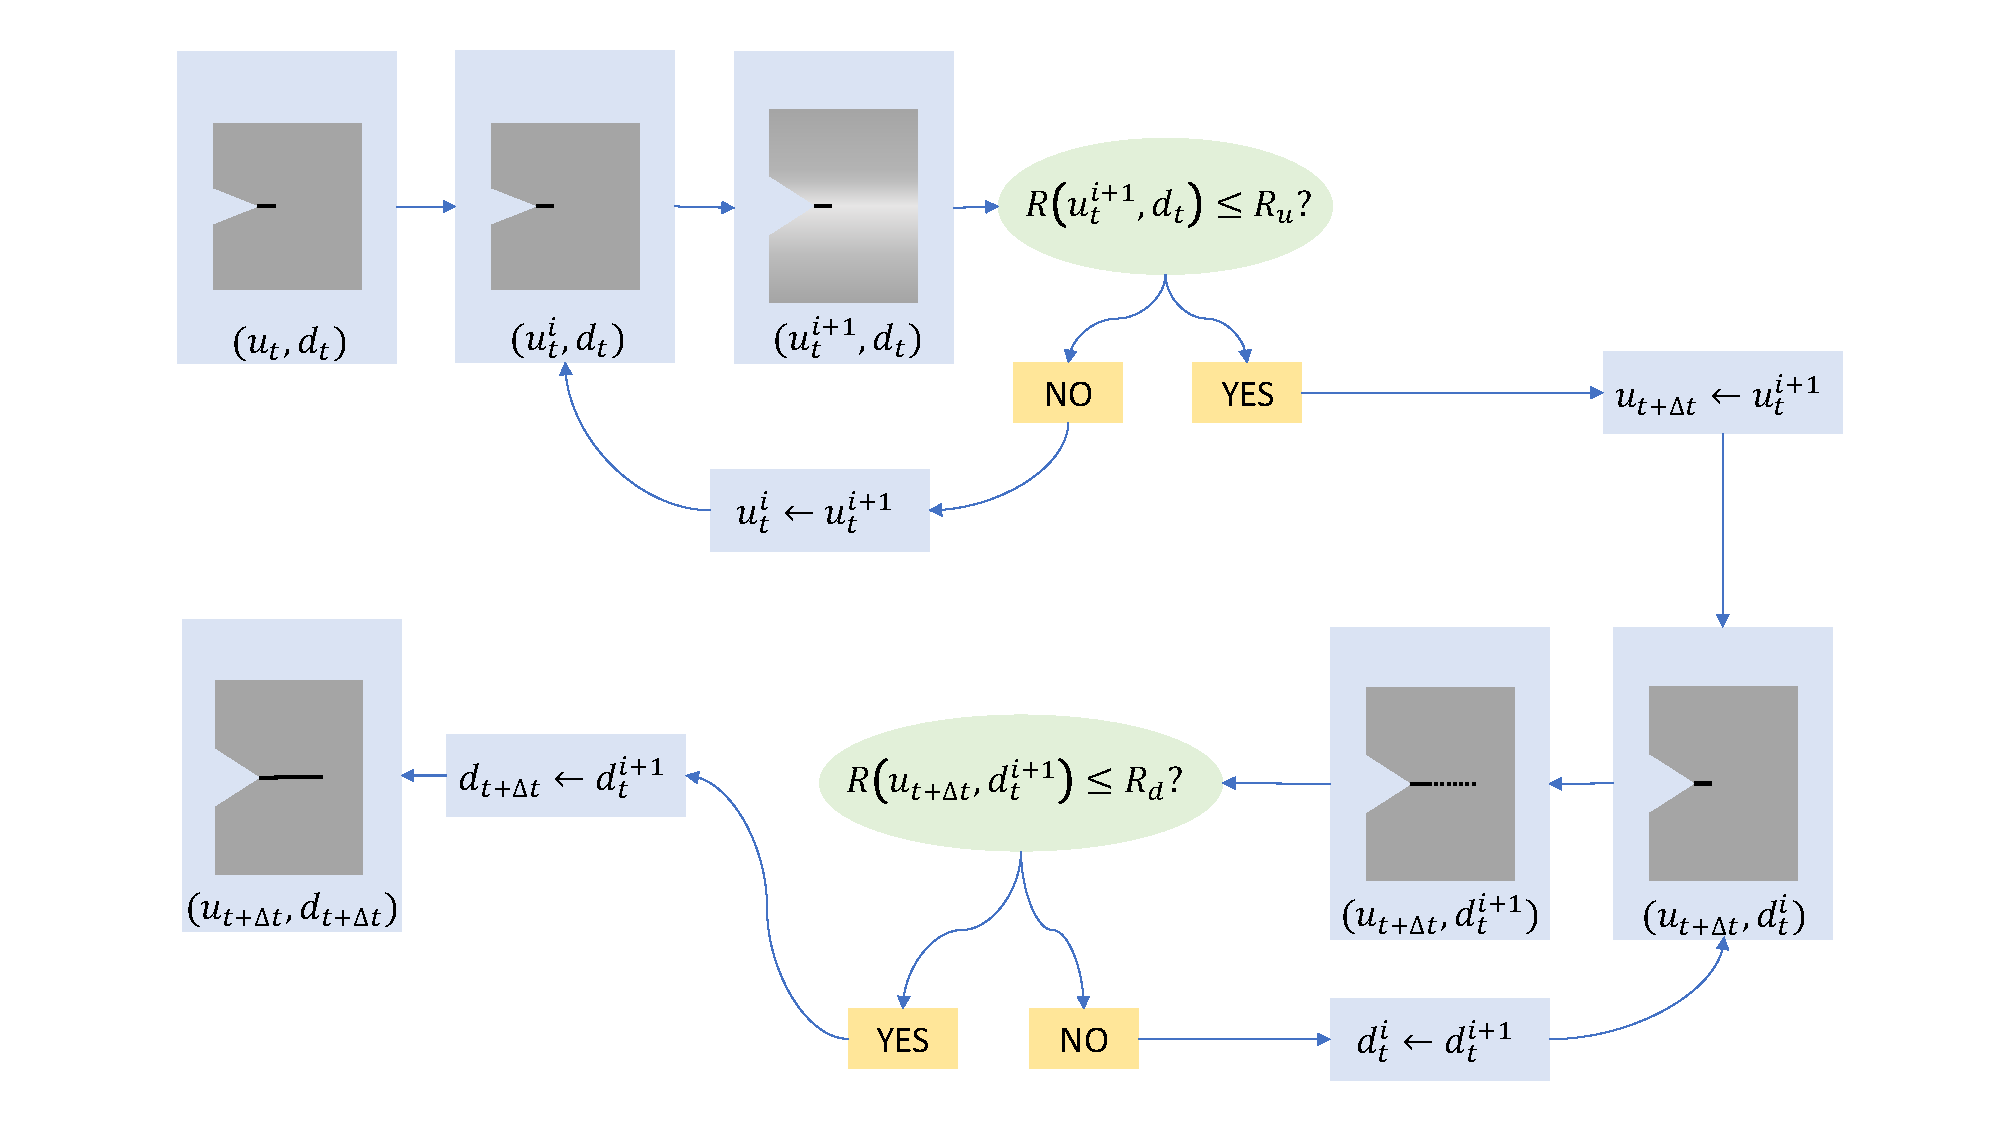
\includegraphics[width=10.cm]{../chapter_00_introduction/figures/time-staggered-resolution.pdf}
  \caption{Illustration of the time staggered resolution of Problem \eqref{eq:phase_field_lagrangian}}
  \label{fig:hho:phase_field:time_staggered_scheme}
\end{figure}

\[
\left\{
\begin{aligned}
  \ets{d}       &= \underset{d^{\star}\geq\bts{d}}{\argmin{}}\, \mathcal{L}\paren{\bts{\vec{u}},d^{\star}}\\
  \ets{\vec{u}} &= \underset{\vec{u}^{\star}\in\text{C.A.}}{\argmin{}}\, \mathcal{L}\paren{\vec{u}^{\star},\ets{d}}
\end{aligned}
\right.
\]

The time staggered approach consists in solving the phase-field problem
with the mechanical state at the beginning of the time step, using the
updated value of the damage field to solve the mechanical problem and
passing to the next time step (see Figure
\ref{fig:hho:phase_field:time_staggered_scheme}).

This approach has been widely used in the litterature
\cite{miehe_phase_2010, nguyen_phase_2015, nguyen_phase-field_2016, molnar_2d_2017, molnar_open-source_2020}.
The results may significantly depend on the loading steps which makes
this approach untractable for our applications.
% as discussed in Appendix
% \ref{sec:phasefield:timestaggered}.

\paragraph{\texttt{Cast3M} implementation}
\label{sec:phase_field:castem_implementation}

The idea that we followed is to integrate the damage update in the
mechanical iterations \cite{helfer_modelisation_2017}, \texttt{i.e.} at each
iteration of the resolution of the mechanical resolution, update the
damage field as follows:

\[
  \ets{d}^{(i+1)} = \underset{d^{\star}\geq\bts{d}}{\argmin{}}\, \mathcal{L}\paren{\ets{\vec{u}}^{(i)},d^{\star}}\\
\]

where \(i\) stands here for the iteration number of the mechanical
resolution.

Note that the convergence guarantees of the alternate minimisation
algorithm are lost.

\paragraph{Work of Ye Lu}

In his postdoctoral work, Ye Lu analysed the previous algorithm and
found that the damage may become almost stationary during the
mechanical iterations \cite{lu_schema_2019}. However, he observed that even
small changes to the damage field perturbates the mechanical resolution,
slowing convergence and even leading to a stagnation of the mechanical
residual. He then proposed to freeze the damage field once it becomes
stationary, a strategy that coined as "semi-implicit". Once the damage
field is frozen, the mechanical problem may be readily solved by a
standard Newton algorithm.

Note that the standard \texttt{Cast3M} algorithm, based on the initial elastic
stiffness, shows poor performance even when the damage field is
frozen.

% <!--
% \subsection{Current status of the \texttt{Cast3M} implementation}

% The \texttt{Cast3M} implementation is currently handles:

% - The Marigo and Miehe treatments of irreversibility.
% - The \texttt{AT1} and \texttt{AT2} phase field models.

% This implementation has been validated using various test cases on the
% literature. The detailed description of all those tests is out of the
% scope of the present report. 

% Figure @fig:phasefield:Cast3MComsol shows the comparison of our
% implementation with an implementation based on the \texttt{Comsol} solver
% developed by the DRT/LITEN and with the results of the original
% implementation by Miehe. Our results compares favourably with the other
% results and highlights the advantage of an implicit scheme over a time
% staggered scheme (see also Appendix @sec:phasefield:timestaggered).

% ![Comparison of the \texttt{Cast3M} implementation of the \texttt{AT2} model with
% Miehe' treatment of irreversibility (on the right) by comparison to the
% results of a \texttt{Comsol} implementation (on the left) on a bending test
% proposed by Miehe \cite{miehe_phase_2010}. Both results matches the result
% of the literature (small figure inlaid in the left figure). Oscillations
% in the \texttt{Comsol} results are due to the time staggered algorithm.
% Courtesy of A. Abaza and J. Laurencin
% (DRT/LITEN)](img/Cast3M-Comsol-Comparison_MieheVersion.pdf){#fig:phasefield:Cast3MComsol
% width=90%}

% ![Fragmentation of an heterogeneous fuel. Extracted from a poster
% presented at the NUMAT conference. Courtesy of V. Gauthier
% (DEN/DEC)](img/poster_vg_0456.pdf){#fig:phasefield:vgauthier width=90%}

% This implementation is already considered in the work of V. Gautier on
% the fragmentation of the MOX fuel (see Figure
% @fig:phasefield:vgauthier).
% -->